\chapter[Distribution of discrete and continuous variables]{Distribution of discrete~and\\ continuous~variables}
\section{Questionnaire (sample)}
%\thispagestyle{empty}
%	\begin{center}
	\fbox{
	\hspace{2em}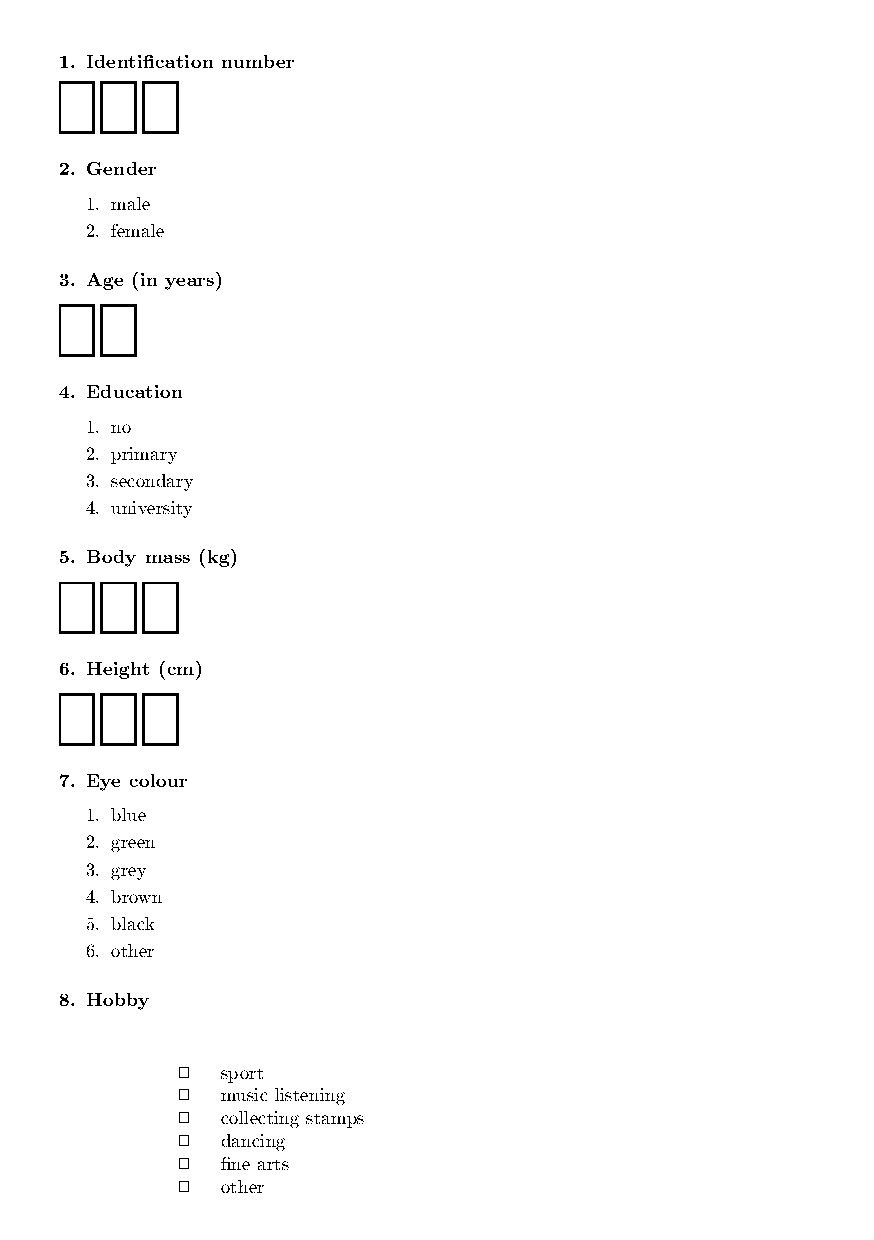
\includegraphics[height=0.8\textheight]{01-kerdoiv.pdf}	\hspace{2em}}
%	\end{center}

\subsection{Create variables using the questionnaire!}

\begin{minipage}{0.48\textwidth}
\centering
	\begin{tabular}{ll}
	\toprule
	variable & type\\
	\midrule
		 ID\\
		 GENDER & categorical, binary\\
		 AGE & \\
		 EDUCATION &categorical, ordinal\\
		 WEIGHT\\
		HEIGHT & continuous, quantitative\\
		  \bottomrule
	\end{tabular}
\end{minipage}
\begin{minipage}{0.48\textwidth}
\centering
	\begin{tabular}{ll}
	\toprule
	variable & type\\
	\midrule
		  E\_COLOUR & categorical, nominal\\
		  SPORT\\
		  MUSIC\\
		  STAMP\\
  		  DANCE&\\
		  FINEART & categorical, binary\\
		  \bottomrule
	\end{tabular}
\end{minipage}



\subsection{Dataset (sample) based on the questionnaire}
\begin{center}
\large
		\begin{tabular}{cccccccccc}
	\toprule
	ID&
	GENDER&
	AGE&
	EDUCATION&
	WEIGHT&
	HEIGHT&
	E\_COLOUR&
	SPORT&
	MUSIC
	\\
	\midrule
	1&1&20&3&65&185&3&1&1\\
	\midrule
	2&2&17&3&60&170&4&1&2\\
	\midrule
	3&1&22&3&62&177&2&2&1\\
	\midrule
	4&2&28&4&62&176&4&2&1\\
	\midrule
	5&1&9&1&32&148&4&2&2\\
	\midrule
	6&1&5&1&19&125&3&2&2\\
	\midrule
	7&2&26&3&70&166&4&2&2\\
	\midrule
	8&1&60&4&75&180&1&1&1\\
	\midrule
	9&2&35&3&49&155&4&2&1\\
	\midrule
	10&2&51&4&61&162&4&2&1\\
	\midrule
	11&1&17&2&61&178&4&2&1\\
	\midrule
	12&2&50&2&65&164&4&2&2\\
	\midrule
	13&1&9&1&30&130&2&1&2\\
	\midrule
	14&2&10&1&40&135&1&2&1\\
	\midrule
	15&1&19&3&86&187&3&1&1\\
	\midrule
	16&1&22&3&67&179&4&2&2\\
	\midrule
	17&1&25&3&103&186&4&1&1\\
	\midrule
	18&1&29&4&74&176&1&1&1\\
	\midrule
	19&2&27&4&67&164&4&1&1\\
	\midrule
	20&1&19&3&70&180&4&1&1\\
	\bottomrule
	\end{tabular}
\end{center}

\section{Discrete variables: distribution, absolute and relative frequency, bar chart}



\subsection{Characterize the \variable{GENDER} variable.}

\begin{minipage}{0.48\textwidth}
	\emph{Frequency table}
	
	\begin{center}
		\begin{tabular}{l|l|l}
		\toprule
				& frequency	&relative frequency (\%)\\
		\midrule		
		male&&\\
		female&&\\
		\midrule
		Total&&\\
		\bottomrule
		\end{tabular}
	\end{center}
\end{minipage}
\hfill
\begin{minipage}{0.48\textwidth}
	\emph{Bar charts (absolute and relative frequencies)}\smallskip
	
	\begin{tabular}{|llll}
	&&\\\\\\\\\\
	\hline
	\multicolumn{1}{l}{}& male && female
	\end{tabular}
	\quad\quad
		\begin{tabular}{|llll}
		&&\\\\\\\\\\
		\hline
		\multicolumn{1}{l}{}& male && female
		\end{tabular}
\end{minipage}
	
	\clearpage
	\subsection{Characterize the \variable{EDUCATION} variable!}

	\emph{Frequency table}
	
	\begin{center}
		\begin{tabular}{l|l|l}
		\toprule
				& frequency	& relative frequency (\%)\\
		\midrule		
		No&&\\
		Primary school&&\\
		Secondary school &&\\
	   University&&\\
		\midrule
		Total&&\\
		\bottomrule
		\end{tabular}
	\end{center}

	\noindent\emph{Bar chart -- (absolute) frequency}\smallskip
		
	\begin{center}
		\begin{tabular}{|llllllllllll}
		&&\\\\\\\\\\
		\hline
		\multicolumn{1}{l}{}& no && primary && secondary && university
		\end{tabular}
	\end{center}
	
		\noindent\emph{Bar chart -- relative frequency}\smallskip
			
		\begin{center}
			\begin{tabular}{|llllllllllll}
			&&\\\\\\\\\\
			\hline
			\multicolumn{1}{l}{}& no && primary && secondary && university
			\end{tabular}
		\end{center}
		
	

%\chapter[Distribution of continuous variables]{Distribution of\\ continuous variables}

%\begin{center}	\begin{tabular}{cccccccccc}
	\toprule
	ID&
	GENDER&
	AGE&
	EDUCATION&
	WEIGHT&
	HEIGHT&
	E\_COLOUR&
	SPORT&
	MUSIC
	\\
	\midrule
	1&1&20&3&65&185&3&1&1\\
	\midrule
	2&2&17&3&60&170&4&1&2\\
	\midrule
	3&1&22&3&62&177&2&2&1\\
	\midrule
	4&2&28&4&62&176&4&2&1\\
	\midrule
	5&1&9&1&32&148&4&2&2\\
	\midrule
	6&1&5&1&19&125&3&2&2\\
	\midrule
	7&2&26&3&70&166&4&2&2\\
	\midrule
	8&1&60&4&75&180&1&1&1\\
	\midrule
	9&2&35&3&49&155&4&2&1\\
	\midrule
	10&2&51&4&61&162&4&2&1\\
	\midrule
	11&1&17&2&61&178&4&2&1\\
	\midrule
	12&2&50&2&65&164&4&2&2\\
	\midrule
	13&1&9&1&30&130&2&1&2\\
	\midrule
	14&2&10&1&40&135&1&2&1\\
	\midrule
	15&1&19&3&86&187&3&1&1\\
	\midrule
	16&1&22&3&67&179&4&2&2\\
	\midrule
	17&1&25&3&103&186&4&1&1\\
	\midrule
	18&1&29&4&74&176&1&1&1\\
	\midrule
	19&2&27&4&67&164&4&1&1\\
	\midrule
	20&1&19&3&70&180&4&1&1\\
	\bottomrule
	\end{tabular}\end{center}

\section{Continuous variables: absolute and relative frequency, histogram}
\subsection{Characterize the \variable{AGE} variable! Create a histogram, make scale on $y$-axis.\\ Interpret the results!}




	\noindent\emph{Frequency table}\hfill\emph{Frequency and relative frequency histogram}
	
	\begin{center}
		\begin{tabular}{l|l|l}
		\toprule
		AGE		& frequency	& relative frequency (\%)\\
		\midrule		
	$\left[0,10\right)$&&\\
	$\left[10,20\right)$&&\\
	$\left[20,30\right)$&&\\
	$\left[30,40\right)$&&\\
	$\left[40,50\right)$&&\\
	$\left[50,60\right)$&&\\
	$\left[60,70\right)$&&\\
		\midrule
		total&&\\
		\bottomrule
		\end{tabular}
%	\end{center}
%
%\noindent
%	\begin{center}
\hfill
\footnotesize
	\begin{tabular}{|llllllll}
		&&\\\\\\\\\\\\\\
		\hline
		\multicolumn{1}{l}{}& 10 & 20 & 30 & 40 & 50 & 60 & 70
\\
\\
\\
		&&\\\\\\\\\\\\\\
		\hline
		\multicolumn{1}{l}{}& 10 & 20 & 30 & 40 & 50 & 60 & 70
		\end{tabular}
	\end{center}

%\subsubsection*{Interpret the results!}
\begin{enumerate}
\item Is the shape of the distribution symmetrical (or skewed)?
\item Which interval contains the most/fewest elements?
\end{enumerate}

\subsubsection*{Double the interval width. Create histograms using data of variable \variable{AGE}. Make scale on $y$-axis.}


%	\emph{Gyakoriság táblázat}
	
	\begin{center}\small
		\begin{tabular}{l|l|l}
		\toprule
		AGE		& frequency	& relative frequency (\%)\\
		\midrule		
	$\left[0,20\right)$&&\\
	$\left[20,40\right)$&&\\
	$\left[40,60\right)$&&\\
	$\left[60,80\right)$&&\\		
		\midrule
		total&&\\
		\bottomrule
		\end{tabular}		
		\hfill\footnotesize
		\begin{tabular}{|llllllll}
		&&\\\\\\\\\\\\\\
		\hline
		\multicolumn{1}{l}{}& 20 && 40 && 60 && 80
		\end{tabular}
		\hfill
		\begin{tabular}{|llllllll}
		&&\\\\\\\\\\\\\\
		\hline
		\multicolumn{1}{l}{}& 20 && 40 && 60 && 80
		\end{tabular}
	\end{center}


\subsection{Characterize the \variable{WEIGHT} variable as done it for variable \variable{AGE}!}

	\begin{center}\small
		\begin{tabular}{l|l|l}
		\toprule
		WEIGHT		& frequency	& relative frequency (\%)\\
		\midrule		
	$\left[0,20\right)$&&\\
	$\left[20,40\right)$&&\\
	$\left[40,60\right)$&&\\
	$\left[60,80\right)$&&\\
	$\left[80,100\right)$&&\\
	$\left[100,120\right)$&&\\										
		\midrule
		total&&\\
		\bottomrule
		\end{tabular}		
		\hfill\footnotesize
		\begin{tabular}{|llllllllllll}
		&&\\\\\\\\\\\\\\
		\hline
		\multicolumn{1}{l}{}& 20 && 40 && 60 && 80 && 100&& 120
		\end{tabular}
	\end{center}
\section{Continuous variables: measures of central tendency and variability}
\subsection{Calculate mean, median, mode, range, standard deviation of these random samples.}\label{subsec:descriptive}

\begin{center}\large
	\begin{tabular}{c|c|c|c|c|c||c|c}
	\toprule
		&$n$&Random sample&
		Mean&
		Median&
		Mode&
		Range&
		Standard deviation\\		
	\midrule
		1.&$n = 4$&1 2 4 1&&&&&\\
		2.&$n = 4$&10 20 40 10&&&&&\\
		3.&$n = 4$&2 4 8 2&&&&&\\
		4.&$n = 4$&2 3 5 2&&&&&\\
		5.&$n = 6$&1 3 2 4 0 2&&&&&\\
	\bottomrule
	\end{tabular}
\end{center}



%\subsubsection*{Compare the mean and the median. Conclude to the symmetry of the distribution.}

\subsection{The numbers of some special operations made by 15 man operators are the following}


	\begin{center}
		20  25  25  27  28  31  33  34  36  37  44  50  59  85  86
	\end{center}	

%The histogram of the sample can be seen below:
	  
	
	\subsubsection*{Based on the shape of the histogram, which statement is true? Why?}
	\begin{wrapfigure}{R}{0.4\textwidth} \vspace{-100pt}
	  \begin{flushright}
	  	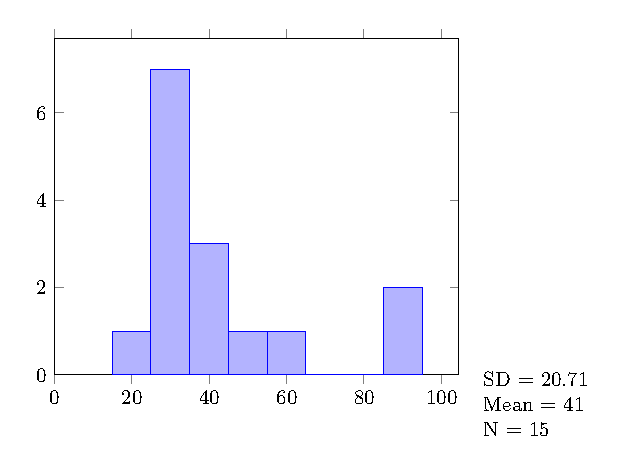
\includegraphics[width=0.36\textwidth]{02-ferfi-operalas}
	  	\vspace{-140pt}
	  \end{flushright}
	\end{wrapfigure}	
	\begin{enumerate}
	\item the mean is smaller than the median
	\item the mean is approximately equal to the median
	\item the mean is greater than the median
	\end{enumerate}

	\subsubsection*{Find the quartiles of the above sample.}
	\begin{enumerate}
	\item first (lower) quartile (25\% percentile):
	\item second quartile (50\% percentile, median):
	\item third (upper) quartile (75\% percentile):
	\end{enumerate}

	\clearpage
	\subsubsection*{Draw a box plot. Compare this to the histogram.\\
		Draw a mean-SD diagram. Can you conclude to the symmetry of the distribution based on this diagram?}
	\vspace{10em}

\subsection{The numbers of some special operations made by 10 woman operators are the following:}


	\begin{center}
	5  7  10  14  18  19  25  29  31  33
	\end{center}	
  	
	\subsubsection*{Based on the shape of the histogram, which statement is true? Why?}
	%The histogram of the sample can be seen below:
	\begin{wrapfigure}{R}{0.4\textwidth} \vspace{-140pt}
	  \begin{flushright}
	  	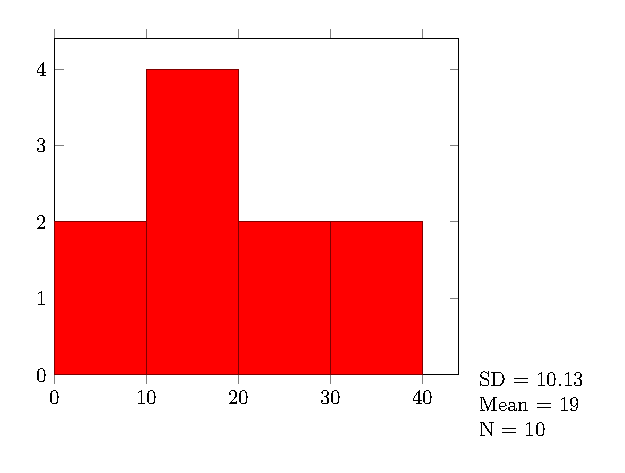
\includegraphics[width=0.36\textwidth]{02-no-operalas}
	  \vspace{-140pt}
	  \end{flushright}
	\end{wrapfigure}	
	

	\begin{enumerate}
	\item the mean is smaller than the median
	\item the mean is approximately equal to the median
	\item the mean is greater than the median
	\end{enumerate}

	\subsubsection*{Find the quartiles of the above sample.}
	\begin{enumerate}
	\item first (lower) quartile (25\% percentile):
	\item second quartile (50\% percentile, median):
	\item third (upper) quartile (75\% percentile):
	\end{enumerate}



	\subsubsection*{Draw a box plot. Compare this to the histogram.\\
	Draw a mean-SD diagram. Can you conclude to the symmetry of the distribution based on this diagram?}
	\vspace{10em}

%\clearpage
\subsection[Putting the diagrams side by side, the two distributions can be compared.]{Putting the diagrams side by side, the two distributions can be compared.\\ Which diagram gives more information and why?}

	\begin{center}
	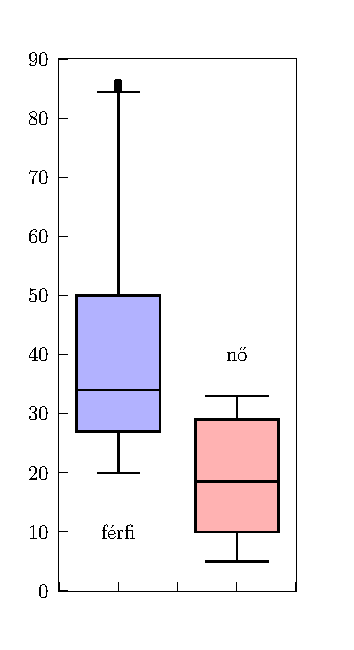
\includegraphics[width=0.15\textwidth]{02-boxplot}
	\hspace{4em}
	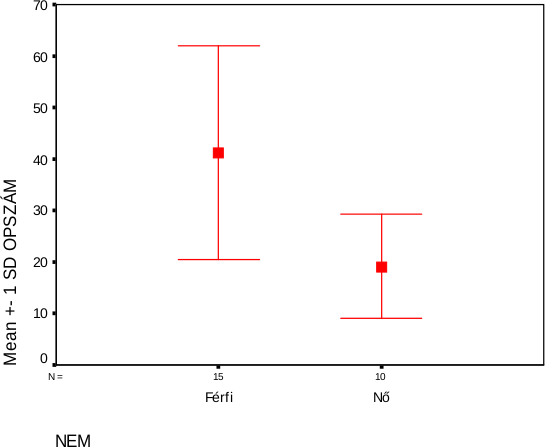
\includegraphics[width=0.2\textwidth]{02-sd}
	\end{center}
	
\section{Calculations with R}

\subsection{Type the samples from the Exercise \ref{subsec:descriptive} in  R and calculate the descriptive statistics.}


\subsection{Open the \data{smallquest\_labels.csv} data file!	
	Repeat the characterization of both \variable{GENDER}, \variable{EDUCATION}, \variable{AGE} and \variable{WEIGHT} variables using the R commands}
	

\subsection{Open the \data{bank.csv} data file. Characterize the continuous variables. Calculate the descriptive statistics of all the continuous variables, e.g. \variable{salnow} (current salary). Interpret the results.}


%\begin{center}	
%	\begin{tabular}{c|c|c|c|c|c|c||c}
%	\toprule
%Variable&
%Min&
%Max&
%Range&
%Mean&
%Median&
%Mode&
%SD\\
%	\midrule
%	&&&&&&&\\
%	&&&&&&&\\
%	&&&&&&&\\		
%	\bottomrule
%	\end{tabular}
%\end{center}


\section{Homework}
\subsection{Here are the blood types of 20 patients. Characterize the distribution of this data.}
	\begin{center}A  0  0  B  AB  0  A  B  B  AB  0  A  0  AB  B  0  AB  0  B  AB\end{center}

\subsection{Given the following temperature values. Calculate summary statistics for the sample, construct a frequency histogram and a box diagram. Conclude to the symmetry of the distribution.}
	\begin{center}35.1  36.1  35.2  36.2  36.5  36.5  37  36.2  36.8  36.7  36.5\end{center}

	
\subsection{Consider the following ordered set of data. Find the mean, first quartile, median, third quartile, range, mode, standard deviation of this data.}
	\begin{center}44  49  50  51  53  57  58  62  66  66  68  71  75  77  80  85\end{center}

	
\subsection{Interpret the results of the table below (Varga Z et al: Individualized positioning for maximum heart protection breast irradion. Acta Oncologica 2013)}

	\begin{center}
	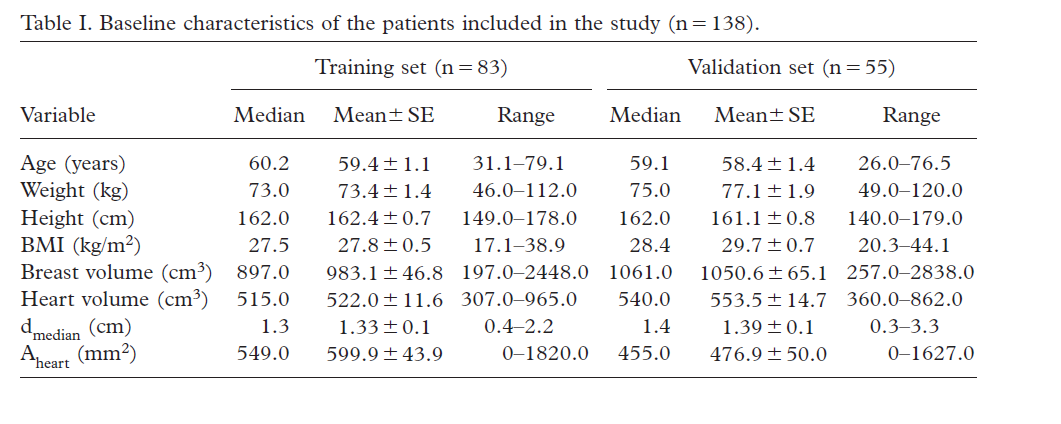
\includegraphics[width=0.7\textwidth]{Adat/02-continuous-table}
	\end{center}
